\chapter{Introduction}
\label{chap:introduction}
\tightlists

As a geneticist, my main goal is to shed light on how genotype results in phenotype. These can be phenotypes at different levels, for example at the cellular level, tissue level or at the organismic level. We know that DNA sets the blueprint for all the phenotypes of an organism at birth. The first and arguably one of the most important steps in the process of going from DNA to phenotypes is gene expression. DNA gets transcribed to RNA and the coding RNA are then translated to proteins. These DNA, RNA and proteins are essentially the molecules that set up life as we know it - both inside us and around ourselves. We function as who we are, our planet is what it is due to the concerted action of these DNA, proteins and RNA.

So, to understand how genotype determines phenotypes it is key to understand gene expression. There are indeed an incredibly large number of research programs around the world devoted to understanding different facets of gene expression. This thesis also attempts to answer a question related to gene expression. Specifically, how is gene expression regulated amongst a population of genetically identical cells that are exposed to the same environment?

Let's peek inside a single-cell. In most cell-types in a human body there are two copies of each chromosome. A small part, about 1\% of this DNA is what codes for proteins \cite {lander2001n}. Through a series of molecular steps that we don't quite fully understand, genes are turned on and off in a precise manner during development across time and space inside an organism. It is this precise turning on and off of genes that generates a whole organism from a single-cell. This precise regulation also underlies the multitude of cell-types and organisms inside and around us. When we hear of such precision, one might think of a well oiled machine that is entirely predictable. A machine that somehow turns on and off in an entirely predictable manner within a cell. Such a machine would perhaps function like a clock, mRNA gets made from DNA at certain intervals of time. But in reality this is not what we observe.

We have become really good at observing and measuring gene expression both in a population of cells \cite{griffith2015pcb}, and within single-cells \cite{macosko2015c, newman2006na, xia2019pnasu, raj2006pb}. If it were true that the gene expression operates in a predictable manner, if we start with a single cell and follow gene expression in it's daughter cells, all the daughter cells would express identical amounts of RNA and protein. However this is not what one observes \cite{elowitz_stochastic_2002}. Cells begin to diverge in their gene expression patterns pretty quickly. Indeed, there is a tremendous amount of cell-to-cell variability in gene expression amongst a population of cells. This thesis deals with understanding this cell-to-cell variability - how does this cell-to-cell variability come about i.e its sources, and does this variability have any phenotypic impact i.e its consequences. Note - In this thesis I use cell-to-cell variability in gene expression and noise interchangeably, they both refer to the same idea.

\section{Gene expression variability exists amongst cells}

Gene expression, where RNA and proteins get made from DNA, is the result of probabilistic interactions between molecules in the cell. These molecules include the two copies of DNA, transcription factors, RNA polymerase, ribosomes amongst others. The low numbers of template DNA, i.e there are only 2 copies of each gene in a cell, involved in transcription results in variable gene expression across cells and time. If on the contrary there were hundreds of copies of DNA it might be possible to predict the average expression of cells using the law or large numbers, and the variability would be smaller. However that is not the case and there is a tremendous amount of molecular variability between cells that gives rise to phenotypic variability between cells. It is still a mystery how even in the presence of these fluctuations  biological systems function in a reliable manner.

The phenomenon of variability between genetically identical cells is however not a new observation. Novick and Weiner \cite{novick_enzyme_1957} \cite{raj_nature_2008} described a phenomenon in 1957 where given a population of E. Coli, the fraction of cells that produce beta galactidase is not deterministic at low inducer concentrations. This fraction varies with the concentration of the inducer. The increase in the concentration of inducer only increases the chance or the probability that a bacterium produces beta galactidase. It looks deterministic after the fact. To elaborate further, given a fixed concentration of the inducer it is not possible to predict with certainty if a single bacterium will produce beta galactidase but it is possible to estimate the probability of this event. This is fascinating. This paper is one of the earliest works that I am familiar with that also talks about variable cell-state amongst genetically identical bacterium - there's an induced state and a non-induced state and the  question is about the transition from one cell-state to another. The authors also compare the enzyme induction state to a mutation because of the phenotypic variability that is observed.

Now let us turn to variability in gene expression. In 2002, Elowitz et al.  \cite{elowitz_stochastic_2002} showed using two-colored reporter genes in E. Coli that identical genes on two different chromosomes show cell-to-cell variability in expression. The authors decomposed this variability into two mathematically independent components. The first is intrinsic noise that is specific to a locus where the gene is located. Intrinsic noise is the result of local interactions of molecules involved in transcription. These might include promoters switching between transcriptionally active and inactive states, proteins such as transcription factors binding to enhancers, recruitment of RNA polymerase to the gene and so on. The second component of variability is extrinsic noise. Extrinsic noise is more global and can be due to differences between cells in what is commonly termed the cellular milieu. The cellular milieu underlying extrinsic noise can include the upstream regulators of transcription such as transcription factor concentrations, number of ribosomes in the cell, differences in cell cycle stage, differences in mitochondrial number etc. These differences in the cellular environment have been shown to affect the expression of multiple genes. \cite{raser_control_2004,blake_phenotypic_2006,blake_noise_2003,raser_noise_2005,volfson_origins_2006}. These studies confirmed the observation, in multiple organisms, that genetically identical cells in the same environment display variability in gene expression

Variability in gene expression has also been observed and modeled at the RNA level. As an example of an early study, in 2006 Raj et al \cite{raj2006pb} counted the number of mRNA molecules of using fluorescence in situ hybridization (FISH). They found a large variation in the number of mRNA molecules between cells of the same cell type. The authors also find that most of the variability they measure is due to intrinsic noise. The authors then modeled the mRNA distributions using a stochastic model of gene transcription and showed that transitions between an inactive state and a state of active transcription, a bursty model of transcription, can explain the observed cell-to-cell variability. They observe variations in burst size, which they attribute to transcriptional activators, but they did not find that the observed data fit changes to burst frequency. This work marked the beginning of a series of studies that used the cell-to-cell variability in the mRNA molecules to understand mechanisms of transcription \cite{symmons2016mc} \cite{chen2018tissues}. The stochastic models of transcription and the estimation of burst frequency and burst size have since become commonly used tools to understand the transcriptional steps that can explain observed cell-to-cell variability under different conditions.

More recently it has also become possible to visualize transcription in live cells. For example, in 2019 Rodriguez et al. \cite{rodriguez_intrinsic_2019} used live-cell RNA imaging to look at the regulation of the estrogen-responsive gene TFF1. The authors observe periods where the gene is transcriptionally active and periods where it is inactive, confirming the bursty model of transcription. An interesting observation however is that the inactive periods vary hugely, they can range from periods that range in minutes to many hours. The active periods are much  shorter and are of the order of 16 minutes on average. It is still unclear what underlies this variability in activation and inactivation. The authors also find instances of allelic coupling where transcription of one allele results in the transcription of the other allele being more likely. Deletion of an enhancer of the gene increases the inactive time period, which agrees with the literature proposing that enhancers control burst frequency \cite{larsson2019n}. The stochastic modeling of the mRNA reveals a deep repressive state  which a gene could spend hours in a repressive state. Using single-cell RNA sequencing data, the authors then postulate that the deep repressive state that is observed for TFF1 could be enriched in genes in certain functional categories such as secretion, trans-membrane and signal peptides. It remains to be seen if this deep repressive state is observed directly in other cells in the future, this paper used observation times of 14 hours which is insufficient to observe this state and this state is a prediction from the stochastic modeling. If this state is real it would be fascinating to understand the mechanisms at the sequence level that underlie this state, again revealing the fascinating ways in which cell-to-cell variability can unveil mechanisms of gene expression.

As we saw in this section with time newer technical innovations have helped us peer at RNA within cells with increasing resolution and they have all revealed that cell-to-cell variability in gene expression is ubiquitous. But does this cell-to-cell variability matter for the cell or is it just a non-functional by-product of how transcription occurs?

\section{Cell-to-Cell variability can result in functional differences}

We know that gene expression regulation underlies the diversity of cell-types that are seen in an organism. Cell-to-cell variability could underlie some of the symmetry breaking where cells undergo different developmental trajectories despite having an identical genome. Indeed an increase in cell-to-cell variability in gene expression has been observed in cells undergoing differentiation. Richard et al.  \cite{richard_single-cell-based_2016} looked at a well-studied differentiation system of chicken erythroid progenitors differentiating into erythrocytes. The authors showed that chicken erythroid cells show an increase in variability of gene expression of relevant genes prior to differentiation. Similar results were obtained by Mojtahedi et al  \cite{mojtahedi_cell_2016} while studying the differentiation of murine heamatopoetic progenitor cells into myeloid or erythroid cells. The authors hypothesize that this surge in variability allows the cells to transition out of stable cell-states and transition to different cell-states. 

Other examples have shown that when differentiation programs are turned on in cell culture models, genetically identical cells don't all reprogram at the same rate. Hanna and Saha et al. showed that reprogramming of somatic cells to iPSCs is stochastic with a random subset of initial cells completing reprogramming  \cite{hanna_direct_2009}. The authors showed that eventually all somatic cells reprogram to pluripotent stem cells when induced with transcription factors but the rate at which cells reprogram can be increased by increasing the cell-division rate. Similar stochasticity has been observed when fibroblasts were reprogrammed into induced endoderm progenitor cells \cite{biddy_single-cell_2018}.

In bacteria, individual bacterium often display a persistor phenotype and grow at slower rates by expressing different subsets of genes. This confers the bacteria an ability to survive adverse changes such as antibiotic treatment that might otherwise terminate a homogeneous population \cite{veening_bet-hedging_2008}. In yeast, variability has been observed in the utilization of the sugar galactose. The Gal genes that are responsible for the metabolism of galactose pathway display a bimodal expression pattern \cite{acar_enhancement_2005}. This bi-modality has been explained using stochastic modelling of the expression of genes in this pathway. 

Variability in phenotype has also been shown to be functionally important at the organismal level. In C. elegans, two identical cells from different lineages known as alpha cells always give rise to exactly one ventral uterine progenitor cell and one anchor cell \cite{seydoux_cell_1989}. Both the alpha cells have the potential to generate either of the two downstream cell-types but which cell becomes the anchor cell is decided in a stochastic and coordinated manner. This case is a well-studied model of a stochastic cell-fate decision where a robust outcome is produced as a result of a stochastic choice. In another example in C. elegans, mutations that cause incomplete penetrance have been shown to be due to increased variability in the expression of cell-fate determining genes  \cite{raj_variability_2010}.  The mutants display increased variability in the expression of a gene called end-1. Cells with high-levels of end-1 are able to activate downstream targets in the intestinal fate specification network whereas the cells with low levels of end-1 do not. We are still at an early stage at uncovering the myriad clinical observations of incomplete penetrance, I'd speculate that cell-to-cell variability in gene expression underlies at-least some of these phenotypes. I discuss more about this in Chapter 4.

Another prominent example of functional effects of variability is the work by Chang et al. \cite{chang_transcriptome-wide_2008}. Chang et al. isolated mouse heamatopoetic progenitors with different levels of a haematopoetic stem-cell marker Sca-1.  Sca-1 expression showed reproducible variability across cells that was not just due to technical error in measurement. The authors used microarrays to show that cells with low amounts of Sca-1 had different transcriptional states compared to cells with low amounts of Sca-1. Furthermore, cells with higher levels of Sca-1 have an increased likelihood of differentiation towards the Myeloid lineage while cells with low amounts of Sca-1 are more prone to differentiate towards the Erythroid lineage. Similar examples have been observed for embryonic mouse cells with different amounts of a stem-cell marker Nanog \cite{kalmar_regulated_2009}. The authors showed that cells with low levels of Nanog exhibit increased variability in gene expression and are prone to differentiate. These results all show how variability in gene expression, often in a single gene, can have functional consequences. 

\section{Noise in transcription factors}

%figure1
\begin{figure}[t!]  
    \centering
    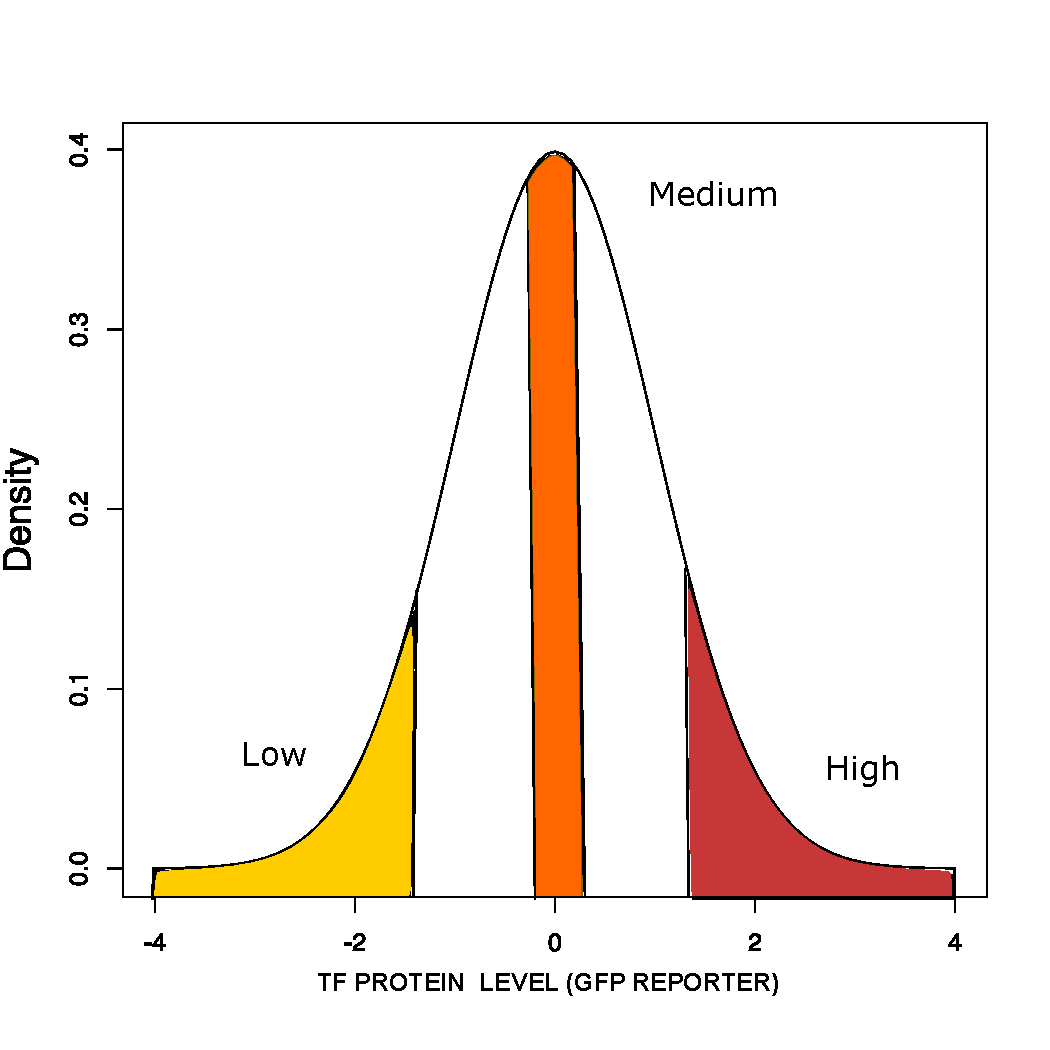
\includegraphics[width=\linewidth, scale=0.25]{figures/intro/intro_gfp_density_X.pdf}
    \caption[Transcription factors display variable expression across a population of cells]{%
        \textbf{Transcription factors display variable expression across a population of cells}
        The protein levels of any given transcription factor is observed as a distribution across cells. In a population of cells, some cells have relatively high amounts of the protein, some have intermediate levels, and some cells have lower amounts of the protein. Does this difference matter?
    }
    \label{fig:intro2}
\end{figure}

Transcription factors play vital roles in development and disease, and can convert between cell-types. \cite{weirauch2011ahotf} \cite{levine2003n}. Consider the distribution in expression of a single transcription factor protein as shown in figure \fref{fig:intro2}. Could it then be that a cell that expresses high amounts of a transcription factor behave differently from another cell, with an identical genome and growing in essentially identical environment, but expressing lower amounts of the same transcription factor? Indeed, several studies have shown this to be the case across different organisms.

Wernet et al. \cite{wernet_stochastic_2006} examined the cell-fate choice in the Drosophila photo receptor cells. The drosophila eye consists of optical units called ommatidia which choose between two sub-types pale and yellow which is determined by the pairs of rhodopsin genes expressed in them. How this fate is chosen amongst genetically identical cells had been a fascinating question. The authors of this paper showed that the expression of a single transcription factor spineless is necessary and sufficient to specify the mosaic cell-fate in the Drosophila eye. Spineless is stochastically expressed in a majority of the cells which then adopt the yellow subtype. The knockout of Spineless results in all of the ommatidia adopting the blue subtype. Overexpressing spineless results in all of the ommatidia adopting the yellow sub-type. This fascinating and crucial development process is thus controlled by the stochastic expression of a single transcription factor.

In \emph{C. elegans} somatic primordium four cells have the potential to be the Anchor cell (AC) which is an important cell in the gonads. \cite{attner2019cb}. How only one of these four cells becomes the AC is determined by the the transcription factor HLH-2. The rest of the four cells become the ventral uterine precursor cells (VU) cells. The relative timing of the expression transcription factor influences cell-fate in this system. The parent that expresses HLH-2 first results in the daughter becoming the VU cell. This onset of expression is also linked to the birth order of the parent cells, the parent cell that is born first also expresses HLH-2 first and adopts the VU fate. However when the birth order difference is  relatively short, the AC/VU decision appears to be random. This system is different from the previous study since it is a stochastic decision while also being a deterministic outcome in that there is always only one AC cell, and this is determined by the birth order of the ancestor cells. The authors speculate that other stochastic outcomes might be resolved by finding other such deterministic elements. 

In Bacteria, Maamar et al. \cite{maamar2007s} examined the emergence of the transient state of competence that enables a bacterium to uptake DNA from the environment. They showed that the noise in comK the master regulator of the competence pathway involving auto-regulation. This auto-regulation results in bi-stability where in one state comK expression is low, and in the other state the comK expression is higher than a critical threshold and enables the bacterium to become competent. They show that the noise in comK is mostly intrinsic.

In this section we have seen several examples across species how the cell-to-cell variability of a single transcription factor can result in important functional differences between cells. In Chapter 2, I present my results where I find that variability in another transcription factor \emph{Prrx1} has functional effects on the hedgehog signaling response. An important follow-up question that emerges from this observation is how can we measure the variability of a given transcription factor. While a whole host of technologies can be used to examine variability I will briefly touch on single-cell RNA sequencing approaches.

\section{Single-cell RNA sequencing approaches to uncover cell-to-cell variability}

In this thesis, I have predominantly used single-cell RNA sequencing to study cell-to-cell variability. Single-cell RNA sequencing allows us to measure the individual transcripts within a cell \cite{macosko2015c}. There are different platforms for performing single-cell RNA sequencing and these have trade-offs in terms of number of cells, number of genes recovered and ease of experimental protocol. The experiments described in Chapter 2 and Chapter 3 use 10X genomics, a droplet based single-cell RNA sequencing technology. In this section I detail how single-cell RNA-sequencing has been used in prior studies of cell-to-cell variability.

A recent study used single-cell RNA-sequencing to estimate the burst frequency and burst size of about 7000 genes genome-wide \cite{larsson2019n}. This study used Smart-seq2 technology which provides coverage across the transcript and shows a reduced 3' bias compared to alternative technologies such as 10X. \cite{picelli2013nm} The authors estimated the average waiting time for a transcriptional burst of a gene is 4 hours though a smaller fraction of genes had waiting times of greater than 20 hours for a burst. Smaller genes have higher burst size, and the authors suggest this is expected for housekeeping genes which are usually compact and consistently expressed in most tissues. Genes with TATA elements also have a higher burst size. By applying their method to a different cell types the authors show that many of the differentially expressed genes between cell-types also show a difference in burst frequency between cell-types. The difference in burst frequency also correlates with histone marks that mark enhancer activity. The authors conclude from these two observations that core promoter elements play a major role in determining burst size and enhancer elements determine burst frequencies and that cell-type specific gene expression is determined by changes in burst frequencies. This sort of genome-wide study of transcriptional kinetics can be enabled by single-cell RNA sequencing and provide a complement to more focused, less noisy assays that look at transcription of a single reporter gene. As the capture technology for scRNA-seq improves we will get better estimates of genome-wide transcriptional kinetics and how they change across different dimensions, for example with genetic background or with age or with disease.

Computational modeling approaches are also very important to understand expression differences between single-cells. The single-cell RNA seq data gives us a static snapshot of a dynamic process such as the cell-cycle or differentiation. A commonly used approach to understand this dynamical process is to cluster cells with similar transcriptomes together. The predicted paths of cellular trajectories are inferred by drawing a principal curve through the cells, and ordering them along this curve which is termed pseudo-time. By correlating the expression patterns along the trajectory with known biology we can infer the processes active in these cells and potentially driving the processes. \cite{trapnell_dynamics_2014}. Another recently developed method called RNA-velocity allows us to infer the near-term future transcriptome of cells. This is done by fitting a kinetic model to the ratio of spliced to unspliced transcripts of each gene. This allows us to estimate the number of inferred transcript counts of different genes. The inferred transcriptome is then plotted on a PCA or tSNE plot to infer the position where a given cell's transcriptome is headed \cite{manno_rna_2018}. Cell state transitions can be modeled as Markov processes \cite{stumpf_stem_2017} and the RNA-velocity approach can be used to infer transition rates of the model. Using such computational models can help answer interesting questions. For example, we can try to understand the proportion of time cells spend in a certain cell-state,  the rate at which a cell can transition to different cell-states, how many cell-states explain the observed data \cite{chang_transcriptome-wide_2008}, the characteristic markers of different cell-states, and what are the genes are driving cell-state transitions \cite{furchtgott_discovering_2017}.

One of the major issues plaguing single-cell RNA sequencing studies is the technical dropout as discussed in detail by several studies \cite{eling2019nrga} \cite{tung2017sr} \cite{hicks2018ba}. Only a fraction of the transcripts (less than 20\%) inside the cell are captured by current single-cell RNA sequencing methods. Further there are amplification biases, especially during the reverse transcription steps which might enhance the noise from dropout. The use of UMIs helps to identify unique molecules of RNA and alleviates some of this issue, but technical variability still remains. Nevertheless, I remain optimistic that these technical challenges will be removed further in the future through experimental and computational innovations and will improve future studies of gene expression noise.

\section{Genetic control of noise}

%figure1
\begin{figure}[t!]  
    \centering
    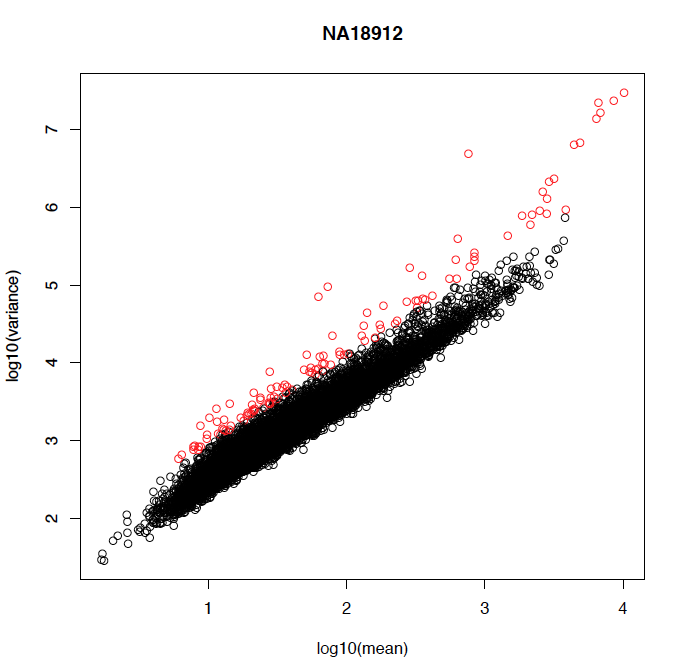
\includegraphics[width=\linewidth, scale=0.25]{figures/intro/intro_outlier1.png}
    \caption[Mean vs variance plot helps identifies genes that are outliers]{%
        \textbf{Mean vs variance plot helps identifies genes that are outliers}
        Using single-cell RNA sequencing data from a YRI individual \cite{sarkar_discovery_2018} I plotted the mean and variance of all the genes. Shown in red are the genes that display a statistically enriched amount of variability than expected according to the mean level of expression. 
    }
    \label{fig:intro1}
\end{figure}

Another important question that still remains to be fully answered is are the mean and noise controlled by different genetic regulatory elements. We have made a lot of progress in identifying loci that are associated with the mean level of expression \cite{gtex_consortium_genetic_2017} \cite{vosa2021ng} \cite{wen2017pg}. These studies have identified eQTLs for almost every gene in the genome and about half of all GWAS hits can now be mapped to eQTLs \cite{gtex_consortium_genetic_2017}. However this only looks at the mean level of expression. Could a similar approach be used to find loci that are variance QTLs? Such an analysis would help identify potential regulatory elements that control the variance.

Studies have looked explicitly for variance QTLs. Sarkar et al. \cite{sarkar_discovery_2018} tried to find variance QTLs using iPSC lines that they generated using the YRI cell lines(n = 53) from the HapMap project \cite{gibbs2003n}. Briefly, they collected single-cell RNA-sequencing data from 54 individuals using the Fluidigm C1 project. Then they fit a negative binomial to each gene and estimated noise measure for each gene. Since they also had genotype information for each of these individuals they looked for variance QTLs. They found all the variance QTLs that they detected were also mean QTLs, indicating that they couldn't find mean independent variance QTLs. The authors concluded that their sample size was too small to detect mean independent variance QTLs and that they would need around 4000 samples to find the strongest mean independent variance QTLs at 80\% power. This study provided methodological innovations to find variance QTLs despite being a negative result. More recent studies such as \cite{resztak2022} have found regulatory elements that are associated with the variance but not the mean. Which subset of the associated loci contains the regulatory elements and how these elements operate is still under investigation.

Prior to the publication of the study by Sarkar et al.\cite{sarkar_discovery_2018} I also looked at the single-cell data generated for this study through a collaboration. I looked at cell-to-cell variability in this data-set using slightly different approaches to the published approach. I looked at every gene's expression separately for every individual, and tried to find genes whose variance in gene expression was disproportionate to their mean levels in that individual. I plotted the observed variance against the mean level for every gene and found a set of genes that had variance above expectation consistently in many individuals (these genes are shown in red in Figure \fref{fig:intro1} for one representative individual). Upon closer inspection, genes that displayed this property were enriched for Mitochondrial genes. We hypothesized that mitochondrial genes might have increased variability for some functional reason. However, it is a known observation in single-cell RNA sequencing that cells that are unhealthy or dying exhibit higher levels of mitochondrial transcripts \cite {stuart2019c}, hence we did not follow up on this observation as this signal could potentially be confounded. We also used this data to look pathways or groups of genes that displayed higher levels of variability than might be expected due to variation in some upstream component of the pathway. However, I did not find any pathways that displayed this property. Like Sarkar et al. I attribute this partly to higher technical noise of single-cell RNA sequencing as well as lower power to detect real effects due to the relatively small sample size of this study. Model organisms have enabled higher sample sizes, and some studies have found regulatory elements that affect the variability. Could these elements be under natural selection?

\section{Selection on noise levels}

From an evolutionary perspective, another question that arises is whether the cell-to-cell variability of different genes are under natural selection, or does selection act only at the mean level. The null hypothesis is that the expression noise is unconstrained by selection and all the selection acts at the mean level of expression. As discussed in the previous section, we are now beginning to identify regulatory elements that are associated with noise but not mean levels. If these regulatory elements are under selection, or if they are conserved across species, these could indicate a possible important functional role for noise that's independent of the mean level of expression of that gene. Many studies have explored this question \cite{lehner2008msb} and I discuss a few of these below.

Newman et al. \cite{newman2006na} measured the noise level for 2500 genes in the the yeast genome under rich and minimal media conditions. They did this by GFP-tagging each gene and measuring the fluorescence level on a cytometer. This collection of GFP-tagged yeast strains has been an invaluable resource, and indeed I used a couple of strains from this project for my early exploratory noise projects that I describe later in this chapter. Newman et al. found that proteins that respond to environmental cues are more noisy than other groups of genes like housekeeping genes. Zhang et al. \cite{zhang2009msb} confirm this observation for plasma transporter genes and use mathematical models to argue that higher noise promotes evolvability of favorable gene expression levels, and suggest that this higher noise could be under positive selection. 

Fraser et al. \cite{fraser2004pb} looked at noise in two classes of genes in yeast - essential genes, and genes involved in protein complex sub-units and compared the noise levels in these two groups to the rest of the genes in the genome. They estimated protein production rates, and transcription rates for every gene in the genome and found that the essential genes and the genes that are part of protein complexes display a lower rate of translation, and a high rate of transcription and decay - a strategy that minimizes noise. The authors speculate that this strategy might have been part of an evolutionary mechanism to minimize noise in genes that are essential to life.

In another study looking at noise in essential genes, Batada et al. \cite{batada2007ng} asked whether genes that are essential are in regions are in regions of the genome that have low nucleosome occupancy, and whether noise-sensitive genes cluster with essential genes in the genome. They reason that genes that are essential might have evolved to be in regions of the genome that are less noisy. Using Myc-tagged histone data they indeed find an anti-correlation between regions of high essential gene density and nucleosome occupancy. They find a dearth of essential genes in sub-telomeric regions which are high noise regions of the yeast genome. Several experimental studies of noise have 

In a study comparing noise in rare vs common variants, Metzger et al. \cite{metzger2015n} looked at the promoter of a yeast enzyme that is involved in glucose metabolism in multiple yeast species. They looked at two classes of variation, polymorphisms that are fixed after undergoing selection through time and new mutations induced through mutagenesis which have not yet undergone selection. They find that the polymorphisms have a slightly smaller effect size on the noise level compared to new mutations, suggesting the action of selection in removing some of the noise affecting polymorphisms in the TDH3 promoter. Naturally occurring haplotypes also show lower amounts noise than what would be expected under neutral evolution. This also suggests selection acting at the noise level.

The studies cited in this section have looked for and found signatures of selection acting on the noise level. However for some of these studies it has been hard to attribute this signal entirely to the variability, and not to the mean level of expression. In the next section we will look at what are some of the genomic features where a gene resides that determines the noise level.

\section{Effect of genomic features and chromatin on noise}

Several studies have looked at the effect of genomic location by integrating the same reporter gene in multiple locations. These studies used sequencing, time-lapse microscopy and flow cytometry approaches to look at bulk RNA and single-cell protein levels in cells. Our approach in Chapter 3 uses a similar integration strategy to look at RNA levels in single-cells to uncover the effects of cellular and genomic environment on gene expression noise.

Akhtar et al. \cite{akhtarw_vansteenselb:ChromatinPosition2013} integrated the same reporter gene in roughly 30000 locations along the mouse genome in ES cells by devising a barcode based technology called Thousands of Reporters in Parallel (TRIP). They measured the mean level of RNA expression of the reporter by using bulk RNA sequencing. Fascinatingly, the expression levels of the reporter genes vary more than 1000-fold in these locations. Nearby locations are correlated in terms of their expression and the authors used a HMM to separate the genome into permissive and non permissive domains. The non-permissive domains overlap with lamina associated domains and late-replicating domains. Permissive IR domains coincide with gene-dense and active regions. The integration locations that are proximal to genes are 10-fold more active than those located far from genes. Our technology in Chapter 3 is highly inspired by the TRIP method of Akhtar et al. The first part of our experimental pipeline is derived from the protocols of Akhtar et al. We wanted to extend TRIP to look at the factors underlying the variance of a reporter gene beyond just the mean.

Dar et al. \cite{dar2012pnas} did a genome-wide study of burst frequency and burst size by using time-lapse fluorescence microscopy at 8,000 loci. The authors use auto-correlation time of the fluctuations as a third axis, apart from mean and noise, to understand the dynamics at different loci. The third dimension allows the authors to constrain the two-state model. They used HIV-1 lentivirus to integrate GFP driven by three different promoters. They find that bursty transcription predominates over constitutive transcription genome-wide. Both burst size and burst frequency vary in equal measure across the genome. Weaker loci modulate the burst frequency to increase expression, whereas after a certain level of expression is reached burst size is modulated to increase expression. They perturbed transcription at this loci using histone deacetylase inhibitors. They find that both burst frequency and burst size increase with increasing expression. 

Dey et al. \cite{dey2015msb} used a lentiviral approach to integrate reporter genes at hundreds of promoters. Their approach used a dual reporter system to quantify the GFP reporter by flow-cytometry and the RNA levels by smFISH. They also assayed chromatin accessibility at the integration sites and found that higher noise locations are enriched for inaccessible chromatin. They also fit a two-state stochastic model to the data and found that the burst size determines the RNA mean while the promoter On-rate influences the noise. This approach by Dey et al. provided a lot of novel insight, however multiple clones had to be measured individually, as a result chromatin analysis was done only on a small set of locations and the locations used in this study were not mapped. A high-throughput approach that allows for potential mapping of thousands of locations would provide more fine-grained insights. Our method in Chapter 3 addresses this limitation.

While all three prior approaches described above furthered our understanding of how mean RNA expression and noise at the protein level changed with genomic locations, there are still some unanswered questions. Can we understand the noise at the RNA level in more locations? How does the cell-state of a cell influence the gene expression noise?

\section{Effect of cell state on phenotypic variability}

In the previous section I discussed the effect of chromatin and genomic features of the location where a gene is situated on expression noise. A complementary factor affecting cell-to-cell phenotypic variability is the cell-state of the cell. As discussed briefly earlier, noise can be decomposed into intrinsic and extrinsic components \cite{swain2002pnas} \cite{raser_noise_2005}. The intrinsic component is related to the fluctuations and biochemical steps involving local transcriptional machinery at the gene being transcribed. The extrinsic component of noise is at the cellular level and varies from cell-to-cell - for example differences in cell-cycle, cell size, number of ribosomes and polymerases between cells etc. A part of this extrinsic component can be captured by measuring the transcriptomes of individual cells \cite{macosko2015c} which is in turn correlated with several cellular components. This set of transcriptional measurements of each cell is also referred to as the cell-state of the cell. Cells of the same type can exist in several different cell-states, though a formal definition of cell-state is still to be determined. Recent studies have begun to examine how the cell-state as captured by the transcriptome affects phenotypic variability between genetically identical cells.

In a study with an intriguing conclusion Foreman et al. \cite{foreman_mammalian_2019} measured the role of cell-state in explaining the amount of phenotypic variability in Calcium signaling after ATP stimulation. The authors used multiplexed error robust RNA fluorescent in situ hybridization (MERFISH) to measure the cell-state of each cell by measuring the mRNA levels of 150 genes mostly related to Calcium signaling and some genes related to the cell cycle. The question that the authors were examining is how much of the variance in the Calcium signaling response can be explained by global factors such as the cell-state, cell-cycle, cell-volume and also differentiation state captured by the transcriptome. They also sought to understand why most gene expression distributions are over-dispersed. The answer is that most of the variability can be explained by cell-to-cell differences such as the cell-state and cell-size. Whatever variability in the expression of a gene remained after accounting for these cell-to-cell differences was Poissonian. This result argues that most of the noise is not gene-specific and that the shared noise dominates the allele-specific noise. This paper offers an intriguing conclusion that transcriptional bursting might not be as prevalent as previously described and that after accounting for the cell-state most genes don't follow a bursty model of transcription. While it remains to be seen how much of this finding translates to other models of study outside Calcium response, it could potentially be important to measure cell-state in any study related to gene expression noise. Our method in Chapter 3 meets this need.

In another study, Torre et al. \cite{torre2021ng} used a genetic screening approach to find genes that regulate a drug-resistant cell-state in cancer cell-lines. This drug-resistant cell-state is initially transient and rare (about 1 in 2000-3000 cells) but upon treatment with drug, this state becomes a stable cell-state.  The authors were interested in understanding what are the pathways that control the emergence of the transient drug resistant state in the first place. They used a genetic screening approach and the authors argue that this approach could potentially uncover genes that are missed in a classic drug-resistance screen, since the phenotype is the emergence of an intermediate state instead of a classic drug resistance screen. They tested two genes identified in the screen DOT1L and LATS2 that increased the frequency of the primed state and another gene BRD2 which resulted in fewer primed cells. Using further validation experiments, they found that the knockout of DOT1L and LATS2 results in larger tumor volumes whereas knockout of BRD2 results in smaller tumor volumes. This sort of genetic-screening approach can help identify the regulators of cell-states that underlie phenotypic variability. One thing that is essential to carry out this sort of approach is some sort of marker of the cell-state one is interested in. In the Torre et al. study they could sort cells based on expression of NGFR and EGFR which mark the primed cells.

In a third complementary study looking at the effect of cell-states on phenotypic variability, Topoleweski et al. \cite{topolewski2022ssb} looked at cell-to-cell heterogeneity in the JAK-STAT signaling pathway response. The authors wanted to test if most of the variability in the signaling response could be explained by differences between cells in their cytoplasmic content, which would reflect their cell-state or if the variability could be explained by just the local intrinsic fluctuations of genes. The authors used an interesting approach by fusing together fibroblast cells to form bi-nuclear synctia. Using this approach, the authors reason that the fused cells could approximate as two separate nuclei with the same molecular content. The authors find that the response of the two nuclei that share the cytoplasm is almost always identical and the shared cytoplasm explains 91\% of the variance in response. The remaining variability is just around 9\%. The authors postulate that the cell-state or the molecular phenotype of a cell could result in the cells interpreting the same signal differently. Thus the phenotypic variability doesn't argue against reliable functioning of single-cells but reflects variability in the content of cells. It still remains to be well understood how the different molecular phenotypes can result in variable outcomes, can we for example predict how a cell will respond to a stimulus using the measured transcriptome information. Such approaches are likely to be possible in the future. In Chapter 3 we devised a new technology that allows us to study the impact of cellular state on the noise level of a reporter gene.

\section{How does noise propagate within a network}

Extrinsic noise as discussed above reflects global cell-to-cell differences such as differences between cells in their cell-cycle, cell-size and affects many genes within a cell. However, it is still not fully clear what are the different levels at which extrinsic noise can act. For example one question we were interested in is can extrinsic noise act at the level of pathways within the cell? This would be reflected in correlated fluctuations in the expression of the genes within a pathway.

One of the questions that I asked early in my thesis work was whether the noise in an upstream regulator of a pathway propagates within the downstream network. The way I tested this was by using one of the GFP-tagged yeast strain for the gene TDH2 from Newman et al.\cite{newman2006na}. TDH2 is an enzyme that is involved in the glycolysis pathway. We hypothesized that protein levels of this enzyme in yeast might manifest as differences in the transcriptomes between yeast (due to differential enzyme activity) and possibly phenotypic differences between yeast. If the noise in TDH2 propagated downstream to the other genes in it's pathway then we would be able to see differences in the target genes when measured by RNA-seq. 

\begin{figure}[t!]  
    \centering
    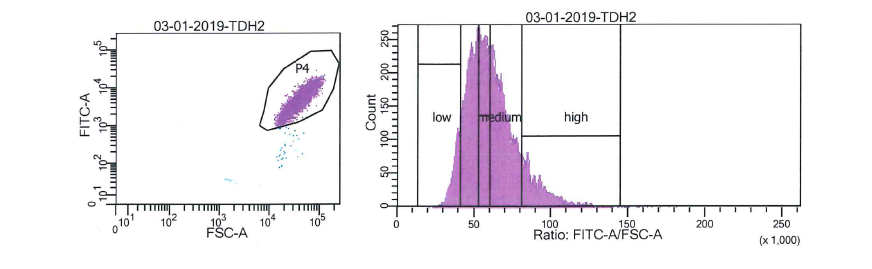
\includegraphics[width=\linewidth]{figures/intro/intro_tdh2_facs.png}
    \caption[Isolation of yeast with different amounts of TDH2]{%
        \textbf{[Isolation of yeast with different amounts of TDH2}
        Yeast with GFP-tagged copies of the gene TDH2 were grown out and sorted on a flow sorter. Three populations of yeast with relative high, medium and low amounts of TDH2-GFP were sorted into individual tubes.
    }
    \label{fig:intro3}
\end{figure}

I sorted out three populations of cells as shown in \fref{fig:intro3}. One population expressed TDH2 at a relatively high level, marked by high levels of GFP, another population at a lower level, and another population of yeast at an intermediate level between the high and low levels.  I sorted these two populations into three separate vials, extracted RNA from the three populations and measured the transcriptomes using RNA-seq.

\begin{figure}[t!]  
    \centering
    \phantomlabel{fig:intro4a}
    \phantomlabel{fig:intro4b}
    \phantomlabel{fig:intro4c}
    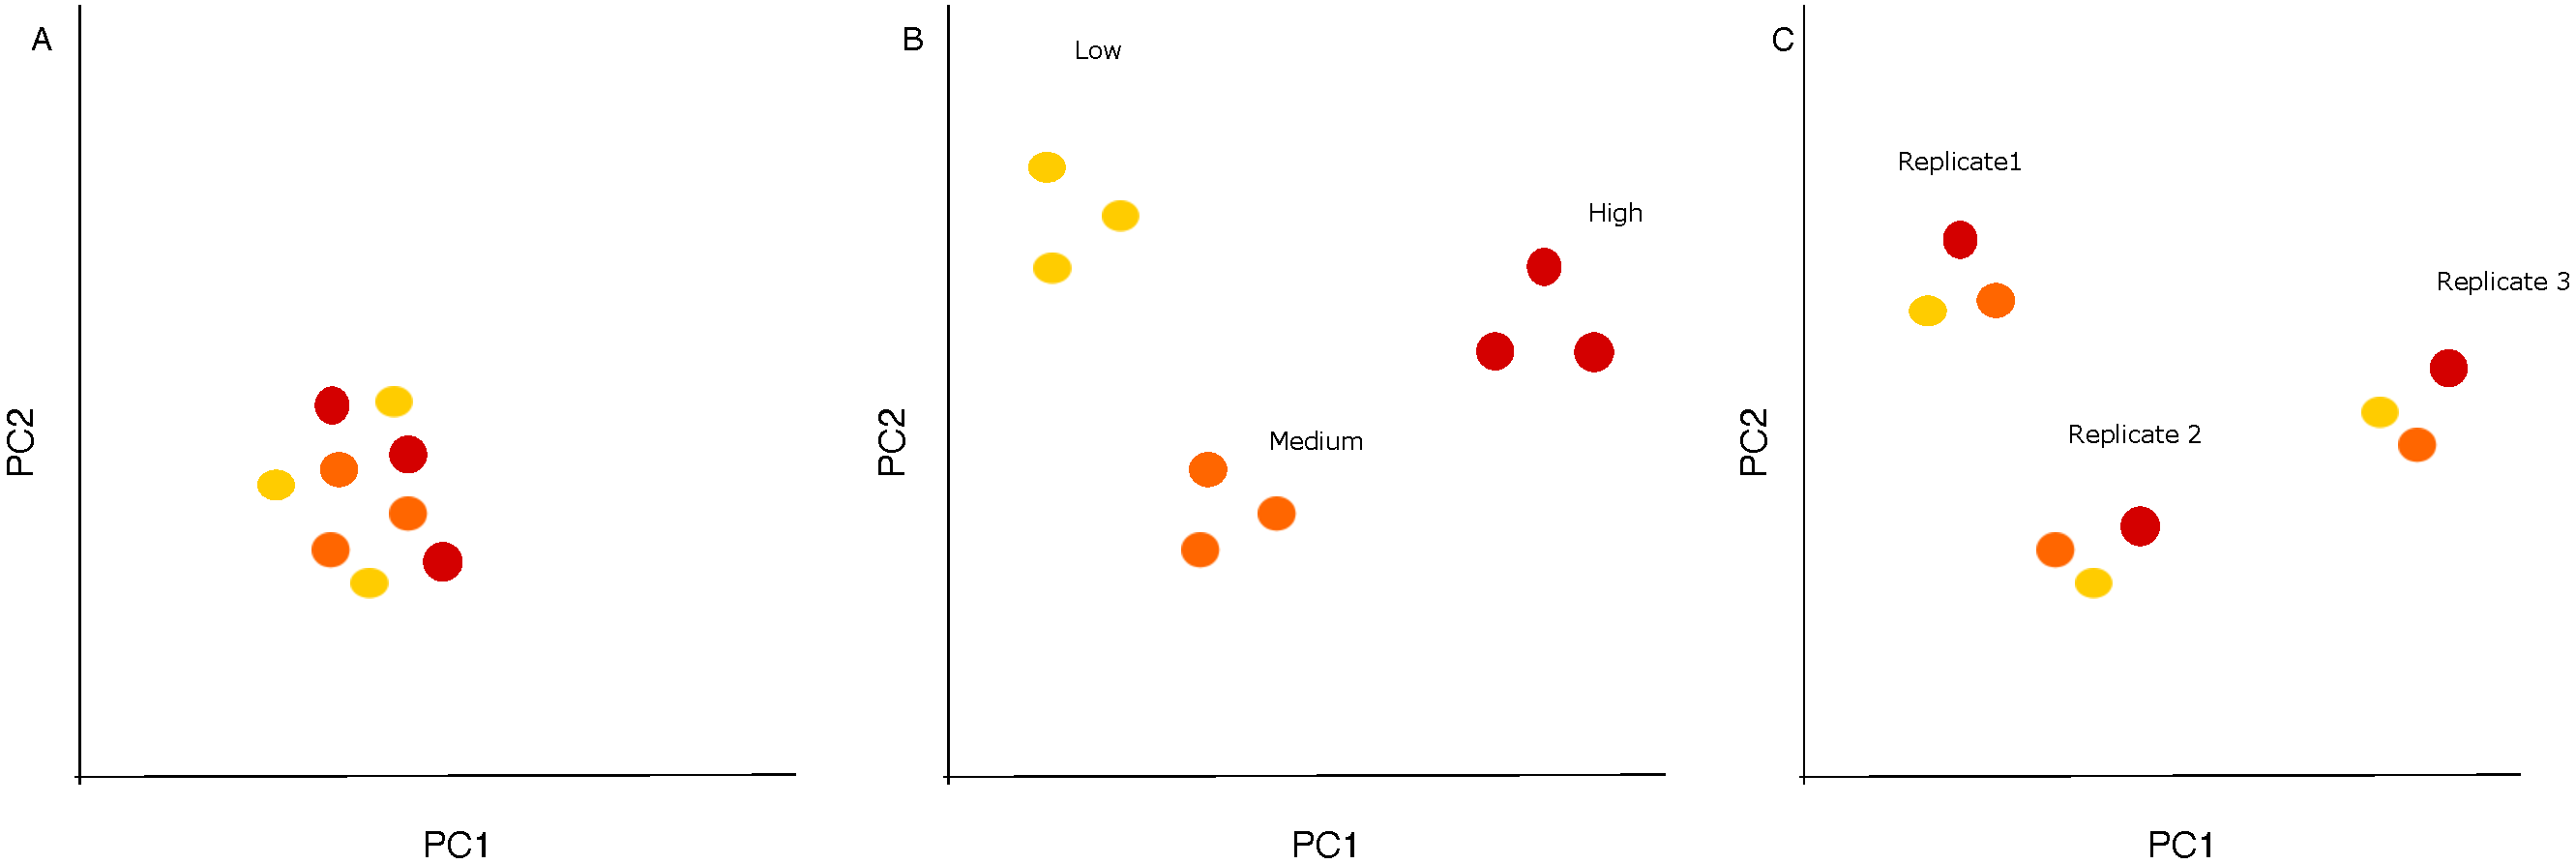
\includegraphics[width=\linewidth, scale=0.5]{figures/intro/intro_clustering_expectedresults.pdf}
    \caption[Expected results using transcriptomes from populations with high, low and medium levels of a protein]{%
        \textbf{Expected results using transcriptomes from populations with high, low and medium levels of a protein}
        A) The transcriptomes don't show any discernible pattern. B) The transcriptomes separate out by the levels of the sorted protein. C) The transcriptomes separate out by a technical factor like batch.
    }
    \label{fig:intro4}
\end{figure}

What might we expect from the transcriptomes obtained from an experiment like this. There are three possible outcomes if we use a clustering analysis like PCA to visualize the data. If the levels of the enzyme did not result in any distinct global transcriptional changes, then we would expect the transcriptomes from the high, low and medium populations to overlap as seen in Figure \fref{fig:intro4a}. If the high and low levels of the enzyme result in distinct transcriptional states, due to up-regulation (down-regulation) of the pathway in the high (low) cells, we would expect to see the results in Figure \fref{fig:intro4b} where the high, low and medium levels of TDH2 result in distinct transcriptional states that cluster separately. This result is similar to what Chang et al see in embryonic stem cells with different levels of Sca-1 \cite{chang2008n}. If the experiment-to-experiment variability i.e batch effects of the experiment dominate the within day variability then we would expect to see the results in Figure \fref{fig:intro4c} where the samples cluster by replicate i.e the day of the experiment. This framework helps us look at the observed data.

\begin{figure}[t!]  
    \centering
    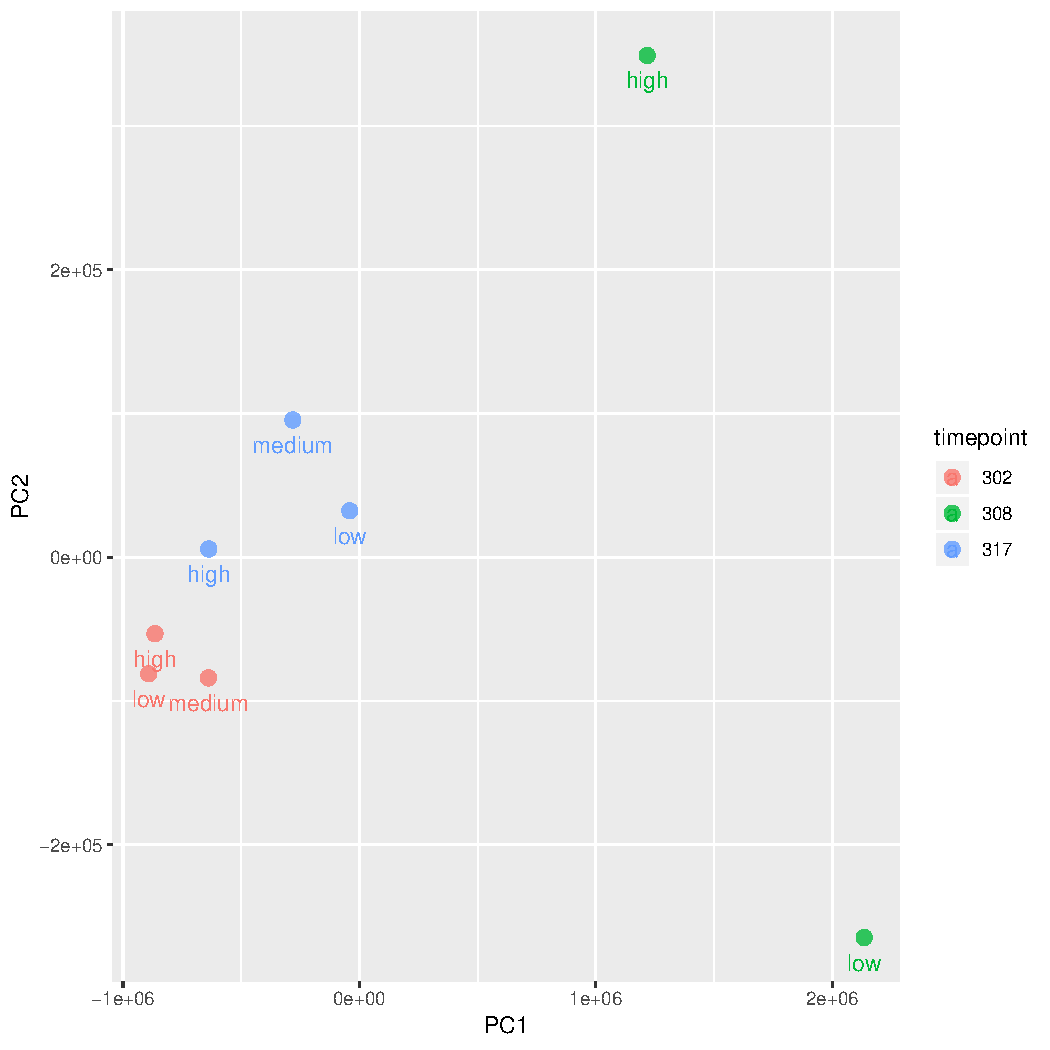
\includegraphics[width=\linewidth, scale=0.5]{figures/intro/intro_tdh2_clustering_timepoints.pdf}
    \caption[Technical variability is greater than biological variability]{%
     	\textbf{Technical variability is greater than biological variability}
     	We sorted out populations of yeast with high, low and medium levels of TDH2 (3 technical replicates each) as shown in \fref{fig:intro3}. We then extracted RNA and performed RNA-seq. We used PCA to visualize the transcriptomes and find that they don't separate out by the sorted TDH2 levels.
    }
    \label{fig:intro5}
\end{figure}

We counted the transcripts for every expressed gene and performed a PCA analysis on the normalized transcript counts. These results are seen in \fref{fig:intro5} The transcriptomes cluster by the day of experiment along PC1. Furthermore, when we looked at individual transcript changes between high and low populations there were very few differentially expressed genes. This result looks like our expected result in \fref{fig:intro4c}. The variability between replicates is higher than the variability within a replicate. Since there were so few differentially expressed genes between the high and low populations we didn't find any pathway related differences between these populations as well.

While this early experiment of mine was largely a negative result I was still able to get started with doing wet-lab experiments and thinking about cell-to-cell transcriptional variability and its possible functional effects. This experiment was technically challenging since large number of yeast had to be sorted in order to obtain enough RNA for library construction. We also had to ensure that the yeast were processed in such a way as to not allow for transcriptional changes after sorting which would remove any real transcriptional differences between the high and low cells. The lessons learnt from this experiment better prepared me for the experiments in Chapter 2 and also inspired me to look for the effect of cell-state on gene expression noise in Chapter 3.

\section{Scope of thesis work}

This thesis consists of two main chapters related to cell-to-cell variability in gene expression. In  Chapter 2 I will try to explain the source of phenotypic variability observed within a cell-type. I will test the hypothesis that cells of the same cell-type express different subsets of genes due to stochastic activation of upstream regulators. Specifically, I will test the hypothesis that stochastic expression of transcription factors and stochastic activation of signaling pathways leads to variability between cells of the same cell-type.

In Chapter 3, I try to understand what determines the noise levels of different genes in the genome. In collaboration with two other graduate students I developed a new genomic technology called SARGENT (Single-cell Analysis of Reporter Gene Expression Noise and Transcriptome) to study noise across genomic locations. Using SARGENT, we integrate the same reporter gene in multiple genomic locations and measure the cell-to-cell variability in expression of this reporter gene using single-cell RNA sequencing. We then attempt to understand the determinants of this noise, after removing the effect of the mean level of expression, using the chromatin state and sequence features at different genomic locations. We also decompose the variability into extrinsic and intrinsic noise, and understand the determinants of these two noise sources. SARGENT also allows us to identify cell-states and quantify the impact of cell-states on noise.
